\documentclass[a4paper,12pt]{report}

\usepackage{cmap}
\usepackage[T2A]{fontenc}
\usepackage[utf8]{inputenc}
\usepackage[russian]{babel}
\usepackage{amsmath,amsfonts,amssymb}
\usepackage{graphicx}
\usepackage{sidecap}
\usepackage{wrapfig}
\usepackage{indentfirst}

\begin{document} 

\begin{titlepage} 

\begin{center} 

\large Федеральное государственное автономное образовательное учреждение высшего образования «Санкт-Петербургский государственный электротехнический университет «ЛЭТИ» им. В.И. Ульянова (Ленина)»\\
кафедра Вычислительной техники\\[5cm] 

\huge ОТЧЕТ\\ по лабораторной работе № 3\\[0.5cm] 
\large <<Обработка двумерных массивов>>\\[3.7cm]

\begin{minipage}{1\textwidth}
    \begin{flushleft}
        \emph{Автор:} Стукен В.А.\\
        \emph{Группа:} 2307\\
        \emph{Факультет:} ФКТИ\\
        \emph{Преподаватель:} Аббас Саддам Ахмед\\
    \end{flushleft}
\end{minipage}

\vfill

Санкт-Петербург, 2022\\
{\large \LaTeX}

\end{center}
\thispagestyle{empty}
\end{titlepage}

\section*{Задание(вариант 13)}
Выполнить обработку элементов прямоугольной матрицы А, имеющей N строк и М столбцов. Исходная матрица состоит из нулей и единиц. Добавить к матрице еще один столбец, каждый элемент которого делает количество единиц в каждой строке четным.


\section*{Постановка задачи и описание решения}
\par
Программа получает на вход количество строк и столбцов матрицы. Затем получает сами значения элементов матрицы.
Далее проходимся по каждой строке матрицы и считаем сумму элементов строки и записываем ее в переменную $count$. Так как исходная матрица состоит только из нулей и единиц, то полученная сумма покажет четность количества единиц в строке. 
Если значение $count$ четное, то в заранее заготовленный массив $b$ размером, равным количеству строк матрицы, 
в $i$ элемент записываем $0$, иначе - $1$. На каждой итерации внешнего цикла(цикла по $i$, который перебирает строки матрицы), обнуляем переменную $count$.
В конце просто выводим элементы матрицы с помощью двух вложенных циклов, в конце каждой итерации цикла по $i$ также выводим элемент $b[i]$.
В итоге получаем матрицу размером $(n,m+1)$ с четным количеством единиц в каждой строке.
\section*{Описание переменных}
\begin{centering}
\resizebox{14cm}{!}{
    \begin{tabular}{|l|l|l|l|}
        \hline
        \textbf{№} & \textbf{Имя переменной} & \textbf{Тип} & \textbf{Назначение}\\
        \hline
        1 & a          &int& Двумерный массив(исходная матрица)\\ 
        \hline
        2 &   n            & int  & Количество строк матрицы\\ 
        \hline
        3 &  m           &  int & Количество столбцов матрицы \\
        \hline
        4 & count        & int & Количество единиц в строке матрицы\\ 
        \hline
        5 & b             & int & Вспомогательный массив, в котором хранятся элементы, \\
    & & &дающие четное кол-во единиц в каждой строке\\
        \hline
    \end{tabular}
}
\end{centering}

\section*{Контрольные примеры}

\begin{centering}
\resizebox{12cm}{!}{
    \begin{tabular}{|l|l|}
        \hline
          \textbf{Входные данные} & \textbf{Выходные данные}\\
        \hline
            3        & 1 0 1 0\\ 
            3        & 1 0 0 1\\ 
            1 0 1    & 0 1 1 0\\
            1 0 0    &        \\
            0 1 1    &        \\
        \hline
            5        & 1 0 1 0 0\\ 
            4        & 1 0 0 1 0\\ 
            1 0 1 0  & 0 1 1 1 1\\
            1 0 0 1  & 1 0 1 1 1\\
            0 1 1 1  & 0 0 0 0 0\\
            1 0 1 1  &          \\
            0 0 0 0  &          \\
        \hline
    \end{tabular}
}
\end{centering}
\newpage

\section*{Примеры использования программы}
    \begin{figure}[h]
        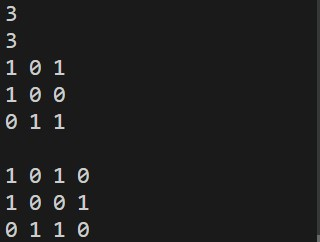
\includegraphics[width=0.5\textwidth]{ex1.jpg}
    \caption{Входные данные 1}
    \label{ris:image}
            
        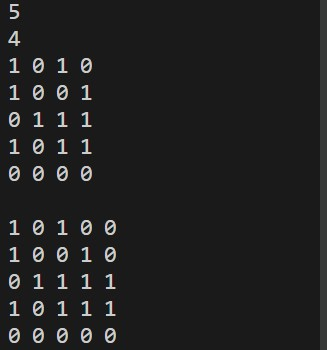
\includegraphics[width=0.5\textwidth]{ex2.jpg}
    \caption{Входные данные 2}
    \label{ris:image}
    
    \end{figure}

\section*{Вывод}
В результате выполнения лабораторной работы изучили работу с двумерными массивами в Си и научились обрабатывать их элементы.

\end{document}